\section{Model Sequence and Geometry-Anchored Texture Learning}\label{sec:models}
\subsection{TREAD-ONE and Motivating Diagnostics}
TREAD-ONE is a 1,372,159-parameter multitask network with $512\times384$ input. A texture encoder and two context transformer blocks support two sigmoid masks, mask-derived boxes, six boundary coordinates, and proxy classification. Twelve nonnegative latent maps contribute to the class logits through a detached, normalized predicted-tread gate and signed class weights.

The three selected seeds achieved strong internal mask agreement but inconsistent proxy transfer. We therefore evaluated a matched seed-1 shared-gradient intervention. Classification is one task and the weighted dense objective the second. When shared gradients have a negative dot product, each is projected away from the other using the original pair of vectors; the projected gradients are then combined. This is a declared symmetric two-task variant motivated by gradient surgery \cite{pcgrad}. It preserves task routing, but global gradient clipping can still affect the total update. Its results do not support promotion over the matched baseline.

ATLAS uses local query and reference features with a frozen dense anchor. ATLAS-LC adds paired local-contrast inputs, excludes identical source images from its 18-image reference bank, and samples with square-root component weights. ATLAS-CONTEXT adds a bounded position-dependent residual to the frozen LC prior. These successive variants provide context for the texture analysis.

GEO, the geometry-first revision, separates geometry, texture, and annotation-error parameters. Its bounded geometry adjustment preserves mask quality and modestly improves internal point error. Its texture representation remains ineligible under the joint gate. A 64-dimensional diversity projector is also difficult to interpret with centered batches of eight, whose covariance rank cannot exceed seven. This dimensional constraint is a feasibility observation, not proof that it caused the failed representation. TRACE retains GEO's fixed final geometry and reduces the auxiliary projector to six dimensions while replacing learned texture targets with explicit fixed descriptors.

\subsection{Canonical Atlas and Fixed Targets}\label{sec:targets}
TRACE uses 1,399,227 frozen geometry parameters and 71,022 trainable texture parameters, for 1,470,249 total. The geometry consists of the selected TREAD-ONE anchor and GEO's final geometry adjustment. GEO's final state was not selected under its original joint gate; its use here is an explicitly frozen research dependency, not a retrospective promotion.

Predicted tyre--tread support defines a canonical $512\times256$ atlas, sampled with bilinear red--green--blue (RGB) values and nearest-neighbor support. Source rows narrower than 16 pixels are unavailable. The atlas contains an $8\times4$ grid of nonoverlapping $64\times64$ tiles. All dimensions in this paper use height before width.

Within each tile, grayscale $g=(R+G+B)/3$ is locally standardized using masked $9\times9$ means and standard deviations, with denominator floor 0.02. The result is clipped to $[-3,3]$, divided by three, and multiplied by observation support to obtain $z$. Tile-local Sobel derivatives $d_x,d_y$, divided by eight, supply edge information. Table~\ref{tab:targets} defines the six fields. These fixed descriptors encode canonical image structure; their thresholds and coordinates have no calibrated physical-wear interpretation.

The four-neighbor Laplacian uses the stencil
\begin{equation}
\Delta z_{u,v}=z_{u-1,v}+z_{u+1,v}+z_{u,v-1}+z_{u,v+1}-4z_{u,v}.
\end{equation}
Thus $\Delta z_{u,v}/4$ is the mean neighbor intensity minus the center intensity in the normalized field.

\begin{table}[t]
\caption{Six fixed image fields before cell averaging. $e=d_x^2+d_y^2$; $\Delta$ is the four-neighbor Laplacian.}\label{tab:targets}
\centering\small
\begin{tabularx}{\columnwidth}{lL}\toprule
Field & Definition\\\midrule
Contrast & $z$\\
Gradient energy & $\sqrt{e}$\\
Orientation axis & $(d_x^2-d_y^2)/(e+0.0025)$\\
Orientation cross & $2d_xd_y/(e+0.0025)$\\
Relative curvature & $\min\{1,|\Delta z/4|/(|d_x|+|d_y|+0.05)\}$\\
Contrast occupancy & $\mathbf{1}[|z|>0.15]$\\\bottomrule
\end{tabularx}
\end{table}

Loss support intersects predicted support with the complement of the annotation ignore mask. An $11\times11$ erosion with invalid padding removes pixels whose radius-five contrast/derivative dependency is not valid. Each tile is reduced to $4\times4$ cells of $16\times16$ pixels. A cell is available only when at least 64 valid pixels remain; the count weights its loss. Missing targets have zero weight and are not treated as observed zeros.

Channel means and population standard deviations are fitted on the 386 training images using 64-bit floating-point (FP64) accumulation and stored in 32-bit floating point (FP32), with a standard-deviation floor of 0.001. Targets are standardized with these statistics. A separate train-position mean is retained for each tile/cell/channel, including its count and availability. Neither statistic uses validation or historical-test targets.

\subsection{Local, Contextual, and Global Paths}\label{sec:architecture}
Figure~\ref{fig:architecture} traces the three readouts. The encoder takes $z,d_x,d_y$, and gradient magnitude as input. Its spatially averaged tile features form the local tokens $Z\in\mathbb{R}^{32\times48}$. A shared tile decoder
\begin{equation}
 D:\mathbb{R}^{48}\rightarrow\mathbb{R}^{96}\rightarrow\mathbb{R}^{96}
\end{equation}
uses a sigmoid linear unit (SiLU) between its two linear layers and reshapes the output to six $4\times4$ fields per tile. Local prediction is $D(Z)$.

\begin{figure*}[t]
\centering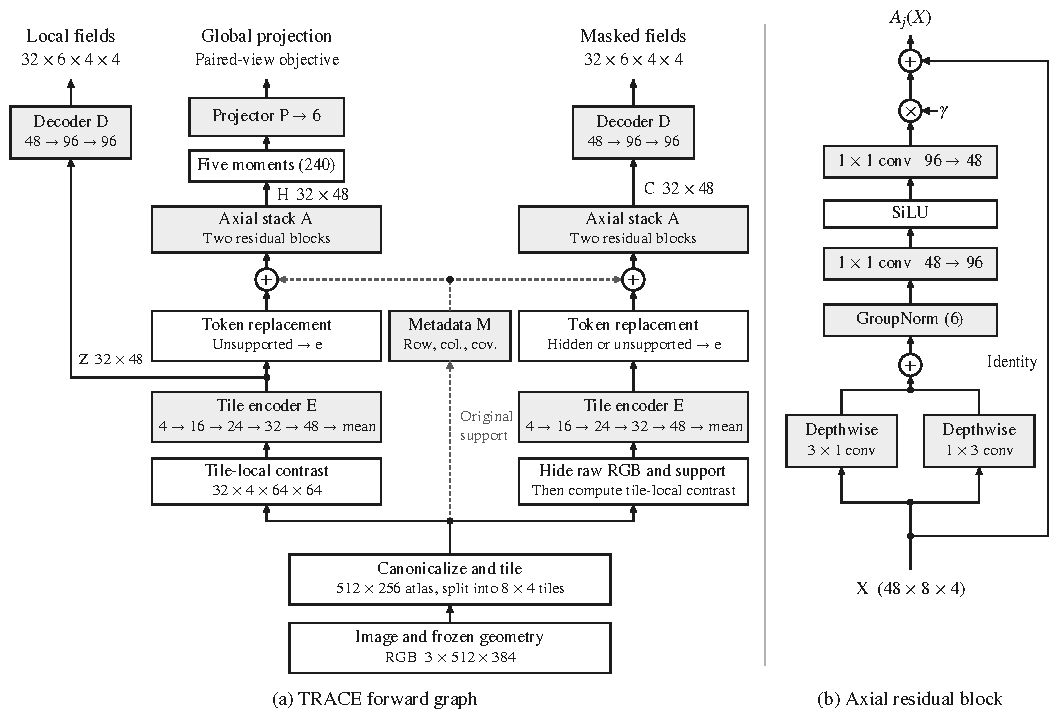
\includegraphics[width=\textwidth]{architecture.pdf}
\caption{TRACE architecture, read from bottom to top. Shading marks parameterized modules. (a) Repeated $E$, $A$, and $D$ symbols denote shared modules. Dashed arrows carry original support and its metadata. The learned mask token is $e$. The five moments use coverage-derived mass. (b) One axial block with per-channel scale $\gamma$ and an identity skip. The two blocks have distinct weights. Batch dimensions are omitted.}\label{fig:architecture}
\end{figure*}

\begin{table*}[!t]
\caption{Exact trainable TRACE layers verified against the executed model source. Tensor sizes omit the batch axis. Encoder shapes are per tile. All convolutions and linear layers include bias. Convolutions use zero padding, GroupNorm uses affine parameters with $\epsilon=10^{-5}$, and both heads use SiLU only after their first linear layer.}\label{tab:architecture}
\centering\small
\begin{tabularx}{\textwidth}{l l L r}\toprule
Layer & Input $\rightarrow$ output & Operation & Parameters\\\midrule
Encoder 1 & $4\times64\times64\rightarrow16\times32\times32$ & $3\times3$ conv., stride 2, pad 1, GroupNorm(4), SiLU & 624\\
Encoder 2 & $16\times32\times32\rightarrow24\times16\times16$ & Same kernel, stride, padding, normalization and activation & 3,528\\
Encoder 3 & $24\times16\times16\rightarrow32\times8\times8$ & Same kernel, stride, padding, normalization and activation & 7,008\\
Encoder 4 & $32\times8\times8\rightarrow48\times4\times4$ & Same blocks, followed by spatial mean to 48 channels & 13,968\\
Metadata & $32\times3\rightarrow32\times48$ & Shared linear projection of row, column, and coverage & 192\\
Mask token & $48$ & One learned vector, zero initialized & 48\\
Axial blocks 1 and 2 & $48\times8\times4\rightarrow48\times8\times4$ & Per block: sum $3\times1$ and $1\times3$ depthwise convs. (48 groups, stride 1, pad $(1,0)$ and $(0,1)$), GroupNorm(6), $1\times1$ conv. $48\rightarrow96$, SiLU, $1\times1$ conv. $96\rightarrow48$, learned scale and skip & $2\times9,888$\\
Tile decoder & $48\rightarrow96\rightarrow96$ & Shared two-layer MLP, reshape output per tile to $6\times4\times4$ & 14,016\\
Global projector & $240\rightarrow48\rightarrow6$ & Two-layer MLP on weighted full-context moments & 11,862\\\midrule
\multicolumn{3}{l}{Total trainable texture parameters} & 71,022\\\bottomrule
\end{tabularx}
\end{table*}

Table~\ref{tab:architecture} specifies the trainable layers. Each context path replaces tiles below 0.25 predicted coverage with the learned mask token. The masked path also replaces intentionally hidden tiles. Both paths add the same projected row, column, and coverage metadata and reuse the axial stack. Its two residual blocks operate on $48\times8\times4$ grids and initialize each learned residual scale to 0.1.

Coverage is normalized within each supported band and then equally across supported bands to yield nonnegative masses $m_t$ with $\sum_t m_t=1$. The recorded local mean is $\sum_t m_t Z_t$, and the full-context mean is $\sum_t m_t H_t$.

The actual global descriptor contains five moments of $H$. Coordinates $y$ and $x$ are the fixed linearly spaced values from $-1$ to $1$ on the eight rows and four columns. With
\begin{equation}
 b_t=[1,y_t,x_t,y_tx_t,y_t^2-1/3],
\end{equation}
the descriptor concatenates $\sum_t m_t b_{tk}H_t$ for $k=1,\ldots,5$, yielding 240 dimensions. The constant $1/3$ is source-defined; the discrete basis is not assumed orthogonal under each image's masses. A $240\rightarrow48\rightarrow6$ projector supplies the paired-view diversity objective. It does not feed the local decoder.

\subsection{Masking, Objective, and Original Selection}\label{sec:training}
Two deterministic image/view-addressed photometric views vary brightness, contrast, and gamma in $[0.9,1.1]$, while targets remain those of the clean atlas. A separate plan hides one supported tile in a band when at least two exist, for at most eight hidden tiles. Hidden raw RGB and observation support are removed \emph{before} preprocessing and encoding. A learned mask token and the permitted position/coverage metadata then enter the context blocks, producing $C$. The masked prediction $D(C)$ is scored on hidden supported cells. Clean targets, annotation ignore masks, and full-path encodings are not context inputs. However, the fixed predicted geometry was computed from the full image; the masking boundary is conditional on that geometry and is not a claim of image-level causal occlusion.

The loss is
\begin{equation}\label{eq:loss}
\begin{split}
\mathcal{L}={}&\mathcal{L}_{\mathrm{local}}+\mathcal{L}_{\mathrm{mask}}
 +0.1\mathcal{L}_{\mathrm{pair}}\\
 &+0.1\mathcal{L}_{\mathrm{var}}+0.01\mathcal{L}_{\mathrm{cov}}.
\end{split}
\end{equation}
Reconstruction uses Smooth L1 with transition $\beta=0.1$ on standardized fields. Valid-pixel counts weight cells, channels are averaged within images, and available images are averaged equally. The two views' terms are averaged. The pair term is mean squared error between six-dimensional projected vectors. With unbiased sample covariance $\Sigma$ ($n-1$ denominator), the variance term averages $\max(0,0.1-\sqrt{\Sigma_{j,j}+10^{-4}})$ over channels. The covariance term is $\sum_{j\ne k}\Sigma_{j,k}^2/(6\cdot5)$. The VICReg-inspired diversity losses require at least seven eligible rows for six-dimensional centered variation.

TRACE uses AdamW with learning rate 0.001, weight decay 0.0001, gradient clipping at one, FP32 arithmetic, and no scheduler or gradient scaler. One seed is run for 60 epochs and 49 updates per epoch. Each epoch has 386 primary image draws and six deterministic padding draws, yielding 23,520 draws in total. Kaggle provides two T4 graphics processing units (GPUs): geometry-cache construction uses the second device and texture optimization the first. This is not distributed data-parallel training.

Three controls predict hidden descriptors: the training channel mean, the training position mean, and the mean of visible descriptors in the same band. All are scored on the same intersection of supported hidden cells and control availability. The original validation contract requires at least 90\% primary exposure and 95\% common control coverage; at least 5\% masked improvement over \emph{each} control; at least 10\% local improvement over the position control; projector rank at least four and median standard deviation at least 0.05; local-mean and spatial-summary ranks at least four; and within-component local/spatial ranks at least two. Finite-state and frozen-geometry provenance checks also apply. Eligible checkpoints minimize masked loss divided by the strongest control loss, plus 0.1 times paired cosine distance, retaining the earliest tie. No epoch is eligible, so the selected endpoint remains unavailable. The final epoch is studied as a fixed diagnostic endpoint.
